\documentclass[onecolumn]{article}
%\usepackage{url}
%\usepackage{algorithmic}
\usepackage[a4paper]{geometry}
\usepackage{datetime}
\usepackage[margin=2em, font=small,labelfont=it]{caption}
\usepackage{graphicx}
\usepackage{mathpazo} % use palatino
\usepackage[scaled]{helvet} % helvetica
\usepackage{microtype}
\usepackage{amsmath}
\usepackage{subfigure}
\usepackage{hyperref}
\hypersetup{colorlinks=true, linkcolor=blue, filecolor=magenta, urlcolor=blue}
\newcommand{\spacecaps}[1]{\textls[200]{\MakeUppercase{#1}}}
\newcommand{\spacesc}[1]{\textls[50]{\textsc{\MakeLowercase{#1}}}}

\title{\spacecaps{Project module report: Argumentation Mining }\\
       \normalsize\spacesc{University of Potsdam, Winter semester 2017/18}}

\author{O\u{g}uz \c{S}erbetci, Maria Stazherova}
\date{\today}

\begin{document}
\maketitle

\begin{abstract}

Structure prediction on ``microtext'' corpus. We used the functional Keras API throughout the project. The code can be found on GitHub at \url{https://github.com/oguzserbetci/argmin2017}.

\end{abstract}


\section{Task \& Data}
Argument mining is the field of study that deals with parsing the structure of the arguments in discourse. The resulting structure helps with the successive analysis and NLP tasks.

In this project our goal was to predict argumentative structures in the
Argumentative microtext corpus~\cite{peldszus2015annotated}, which contains 112 short argumentative texts
(originally in German and professionally translated to English).
We also received preliminary annotations of the new microtexts
and could incorporate them into the project.

\begin{figure}[h]
    \centering
    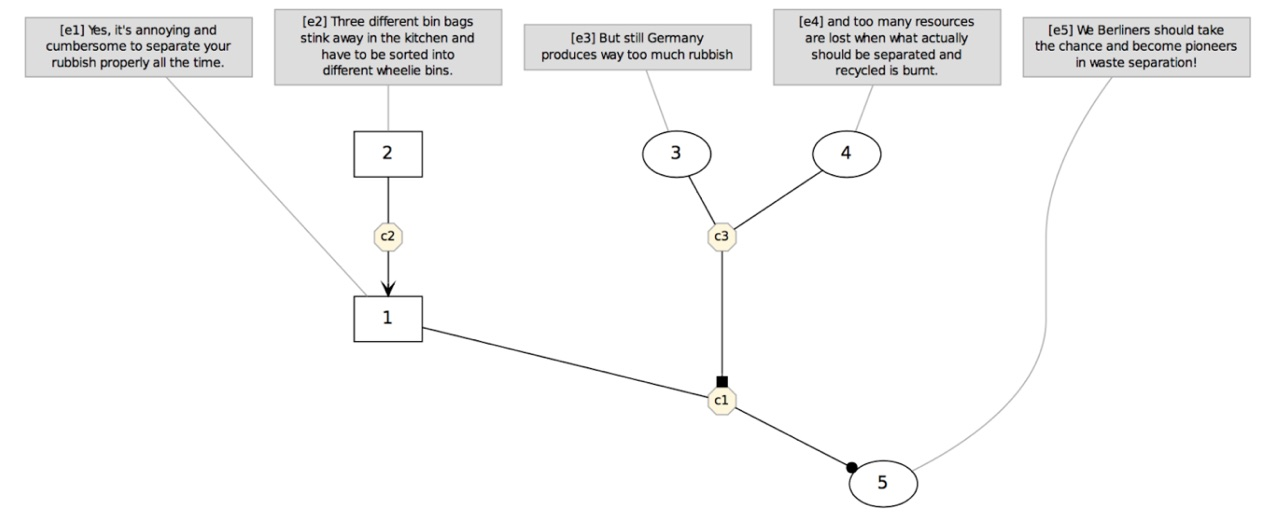
\includegraphics[width=0.8\linewidth]{fig/microtext.jpg}
    \caption{One example from arg-microtext corpus and its argumentation graph.
            \\Round nodes are proponent's nodes, square ones are opponent's nodes.
            The arcs connecting the nodes represent different supporting and attacking moves.}\label{fig:microtext}
\end{figure}

As seen in the figure~\ref{fig:microtext}, each text in the corpus is a single tree made up of argument components (ACs), of which one is the claim and the rest are premises.
We decided to concentrate on two tasks: classifying the type of an AC (claim or premise), and determining the links between ACs.

\section{Approach}
\subsection{Inspiration}
Having found the paper ``Here's My Point: Joint Pointer Architecture for Argument Mining'' by Potash et al.~\cite{potash2017here}, we agreed that it
would be good to try and reproduce the architecture and the results from this paper, especially because the authors claimed they achieved
state-of-the-art results. The authors use a Pointer Network~\cite{pn} which is a modification of seq2seq (sequence-to-sequence) architecture~\cite{seq2seq} with attention~\cite{attention}.

In~\cite{potash2017here}, authors limit the problem of argument mining to following scenario:
Given a set of ACs, predict the argument structure by predicting the links between ACs.
To this end, the pointer network architecture is extended in two ways.
First, to account for the large and sparse AC representations, fully-connected layers are added before the encoder and decoder LSTM inputs.
Second, an auxiliary task is added to improve performance. The task is to predict whether an AC is the claim or a premise.
Note that this task is redundant because the root of the tree, which can be inferred from the argument structure, is always the claim.
However, multi-task learning in deep neural networks has been shown to perform better in comparison to single task~\cite{multi}, which the results of this work further demonstrates.

\subsection{Architecture}
The architecture from \cite{potash2017here} is a seq2seq model as depicted in~\autoref{fig:seq2seq}.
For brevity let us leave out the fully connected layers before the inputs of the encoder and the decoder.
At each time step, an $\text{AC}_i$ is input into the encoder and results in hidden state $e_i$,
which is then used to predict the probability distribution over whether the $\text{AC}_i$ is the claim or premise.

\begin{align*}
    z_i = W_{\text{cls}} e_i + b_{\text{cls}}\\
    p(T_i|E_i;\Theta) = \text{softmax}(z_i).
\end{align*}


After the final AC has been input into the encoder, the decoder has its first time step.
The first input to the decoder is always the special start token and results with the hidden state $d_1$.
At each decoder time step the modified attention mechanism outputs the probability distribution over links as follows:
\begin{align*}
    u_j^i &= v^\top \tanh(W_1e_j + W_2d_i)\\
    p(D_i|D_1,\dots,D_{j-1},E) &= \text{softmax}(u^i).
\end{align*}

The model for the type and link predictions are depicted in~\autoref{fig:type} and~\ref{fig:link}.

\begin{figure}[h]
    \centering
    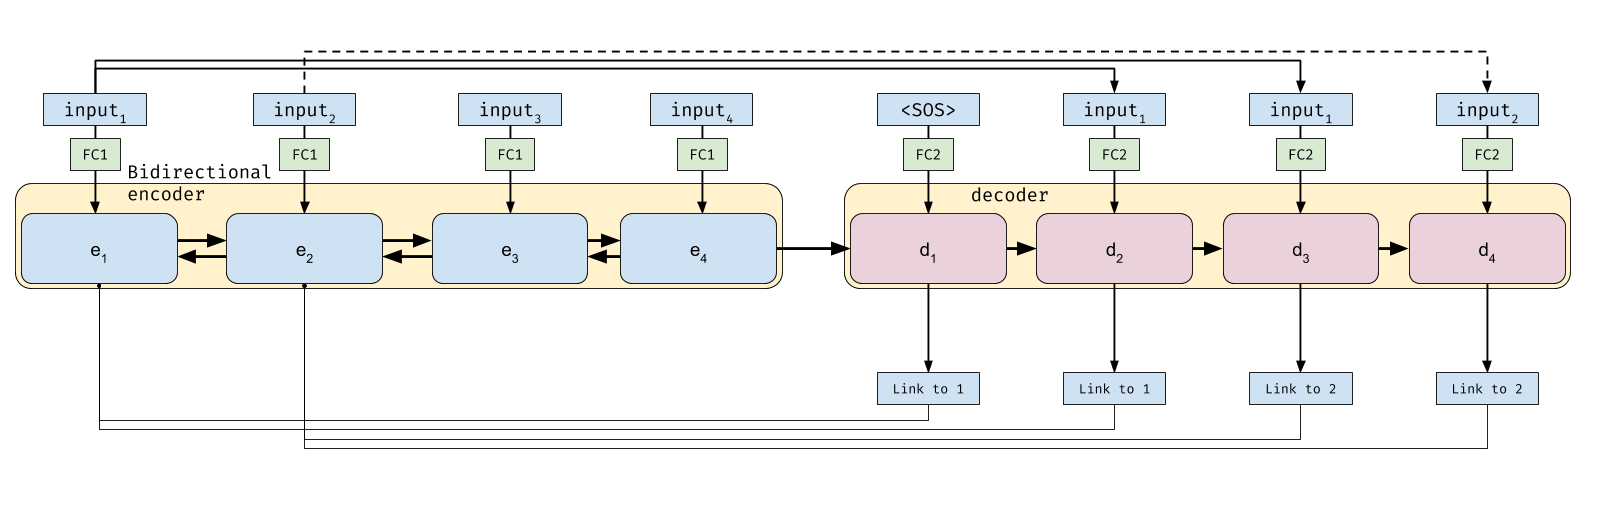
\includegraphics[width=0.8\linewidth]{fig/seq2seq.png}
    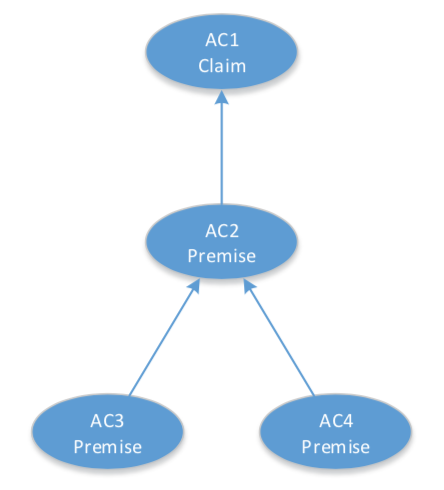
\includegraphics[width=0.18\linewidth]{fig/acs.png}
    \caption{Seq2seq architecture of Pointer Network on the left and the predicted argument structure with 4 ACs on the right.}\label{fig:seq2seq}
\end{figure}

\begin{figure}[h]
    \centering
    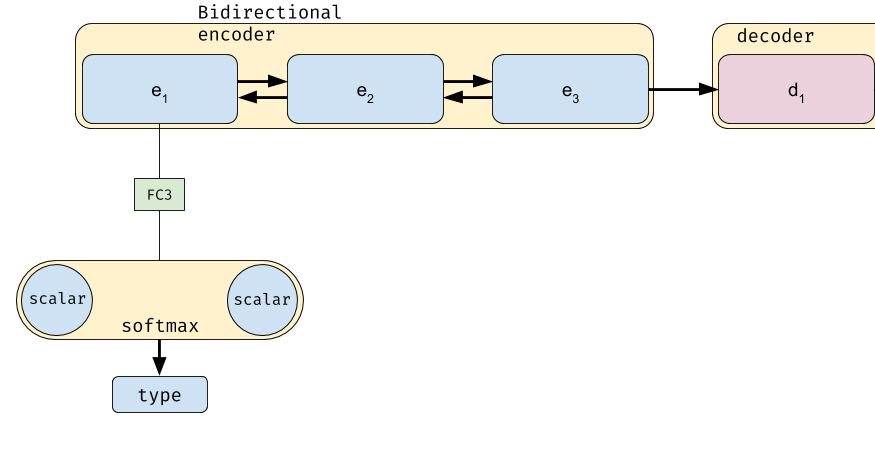
\includegraphics[width=0.8\linewidth]{fig/type.png}
    \caption{Diagram of the model for predicting type of $\text{AC}_1$. FC3 is a single fully connected layer that is being applied to each AC to predict the type.}\label{fig:type}
\end{figure}

\begin{figure}[h]
    \centering
    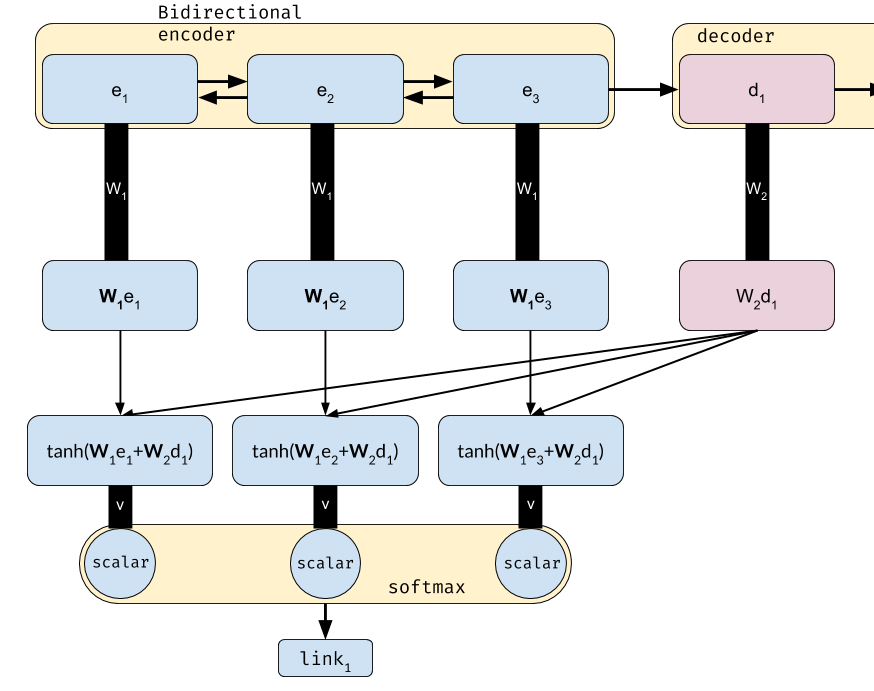
\includegraphics[width=0.8\linewidth]{fig/link.png}
    \caption{Diagram of the model for predicting the outgoing link from $\text{AC}_1$. Thick edges represent a dot product with a parameter matrix.}\label{fig:link}
\end{figure}

\subsection{Implementation \& Organisation}
For embedding the ACs we have used spacy w2v models and the sklearn's bag of words featurizer.
The seq2seq model was implemented with Keras functional API

We have organized the project into 3 milestones and enforced deadlines.
In milestone 1, we have implemented the data preprocessing and created simple bag-of-words vector representations of argument components.
After that we implemented a pointer network with one-directional encoder for the single task (determining the links between ACs) without the fully connected layer at inputs.
We sticked to using $0.9$ dropout, as it was specified in~\cite{potash2017here}.
However, because the paper didn't specify where the dropout should be used, we had to do a hyper-parameter search.

In milestone 2, we extended the architecture with the fully-connected inputs and the bidirectional LSTM for the encoder.
Moreover, we have added all applicable features to AC representation from the paper: the structural feature
(binary, if the AC is the first one in text or not), the bag-of-words representation and the embedding representations (average, min and max pooling
of word vectors\footnote{We have used \href{https://github.com/explosion/spacy-models/releases/tag/en_vectors_web_lg-2.0.0}{spacy} word vectors.} of tokens).

In milestone 3, we have implemented the joint model architecture with the auxiliary task of classifying the type of AC (claim or premise).

During development, we have used 5-fold cross-validation to evaluate different configurations and inspect our implementation.
Some things we had to try out were: using weight decay (l2 regularization), where to apply dropout and the seq2seq architecture.
Weight decay did not improve performance when applied as an addition to dropout.
Using only weight decay instead of dropout also performed worse compared to dropout.
We found that dropout works best when applied to LSTM's cell state and input and nowhere else.

\subsection{Challenges}
While working on the project, we encountered some difficulties and made some errors that we then corrected. The first one
was to think of the proper way to pad input sequences so that they have the same length.

Our biggest mistake was to implement the seq2seq architecture without the decoder inputs and to stack the encoder and the decoder on top of each other. Surprisingly this did not effect the performance much.

Another mistake we did was to calculate the evaluation metrics wrong.
We have calculated the f1 score not as a binary classification of absence and presence of links, but as a categorical one instead.
This has resulted in significantly worse results which led us to tinker with our architecture and identify the wrong seq2seq architecture. We have even implemented the architecture in pytorch from scratch.

This mistake and its correction has been a great learning for us, however, we note that the binary measure makes the results look much better than they are,
since by definition in the worst case for $n$ ACs the network gets $n-2$ absence of links correct. Therefore, taking the macro average of the binary f1 score is misleading. We think the result that most telling is the f1 score for the prediction of the presence of links.

Finally, when we parsed the new corpus, we had to account for the inconsistent indexing scheme.

\section{Results}
To compare our results we did a 10-fold cross validation. Our results and the results from~\cite{potash2017here} can be seen in~\autoref{tab:res}.

\begin{table}[h]
    \centering
    \begin{tabular}{| l || c | c | c | c | c | c |}
        \hline
        & \multicolumn{3}{|c|}{Type prediction} & \multicolumn{3}{|c|}{Link prediction} \\ 
        \hline
        Model & Macro f1 & Cl f1 & Pr f1 & Macro f1 & Link f1 & No Link f1 \\
        \hline
        Their Joint Model                 & 0.813 & 0.692 & 0.934 & 0.749 & 0.577 & 0.903 \\
        Our Joint Model                   & 0.824 & 0.714 & 0.934 & 0.737 & 0.526 & 0.947 \\
        Our Single Task Model             &   –   &   –   &   –   & 0.755 & 0.559 & 0.951 \\
        Our Joint Model with new data     & 0.809 & 0.695 & 0.922 & 0.716 & 0.516 & 0.943 \\
        Our Joint Model with loss weights & 0.806 & 0.699 & 0.913 & 0.725 & 0.505 & 0.945 \\
        \hline
    \end{tabular}
    \caption{The results of 10-fold cross-validation of different configuration of our model.}\label{tab:res}
\end{table}

Our results presented in \autoref{tab:res} are similar to ones reported in~\cite{potash2017here}, which we include in the table for convenience.
One interesting observation is that our single task model had better performance on link prediction in contrast to results reported for the Persuasive Essay corpus in \cite{potash2017here}
(\cite{potash2017here} does not include the single task performance on the microtext corpus.)

We also present results from the new extended corpus.

Another additional configuration we present is to apply class weights as a weight to loss calculation.
We were motivated to use class weights because of the highly skewed link and type distribution across the corpus as seen in~\autoref{fig:skew}.
As seen in \autoref{tab:res} this worsens the performance.

\begin{figure}[h]
    \centering
    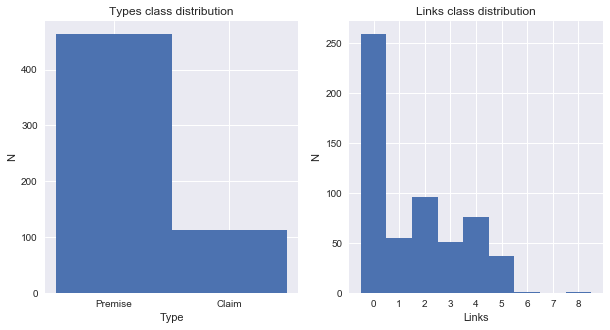
\includegraphics[width=0.6\linewidth]{fig/dist.png}
    \caption{Distribution of links.}\label{fig:skew}
\end{figure}

\section{Conclusion}
We have learned a lot through this project.
The implementation was not as straight forward as we have thought it would be.
There are many possible future extensions we would have liked to do.
First, as the authors have suggested in~\cite{potash2017here}, using a seq2seq model to embed ACs might improve the performance greatly.
It would also eliminate the need for the fully connected layers that add a lot of unnecessary model complexity.
However, a seq2seq representation of ACs would require much larger data.
We suggest using a large unannotated corpus with sent2vec or transfer learning as described in~\cite{sent}.

Another extension is to build an end-to-end architecture which can identify ACs in a text.
We think that these two extensions are intertwined and should be explored together.
Because solving this task would require large amounts of data and transfer learning.

An easier extension would be to add even more tasks to see if it helps with performance.
The microtext corpus already has additional information that can be used such as the role of the AC, and the function of the AC.

Another note for future work would be to use a deep learning framework with dynamic graphs like pytorch or dynet.
We have tried it shortly and found it to be a much better fit for a seq2seq model.

\nocite{*}
\bibliographystyle{plain}
\bibliography{references}
\end{document}
